\begin{anexosenv}

\partanexos

\chapter{Canvas}

  \begin{figure}[!htb]
    \label{canvas}
    \centering
    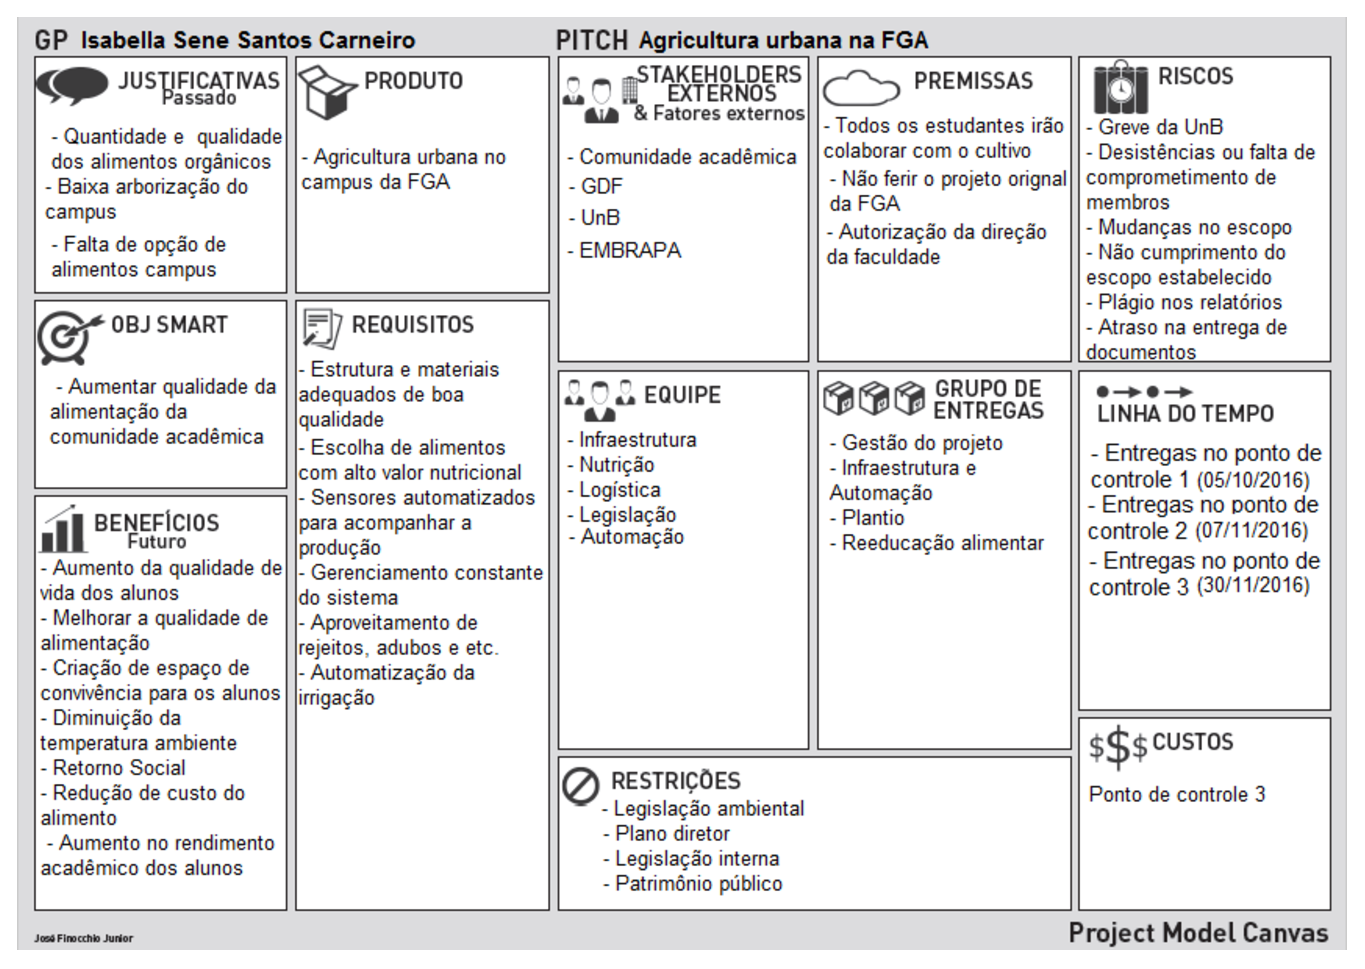
\includegraphics[width=17cm, keepaspectratio=true]{figuras/introducao/canvas.eps}
    \caption{Canvas de projeto}
  \end{figure}

\chapter{Distribuição das equipes}

  \begin{table}[!htb]
    \label{equipes}
    \centering
    \begin{tabular}{p{7cm}p{3cm}p{3cm}}
      \toprule
        \textbf{Nome} & \textbf{Função} & \textbf{Área} \\
      \midrule
        Isabella Sene Santos Carneiro & Gerente    & $-$            \\ \midrule
        Allan Jefrey Pereira Nobre    & Subgerente & Infraestrutura \\ \midrule
        Milena Martins Magalhães      & Subgerente & Nutrição       \\ \midrule
        Caue Mateus Oliveira          & Subgerente & Legislação     \\ \midrule
        Victor Hugo Arnaud Deon       & Subgerente & Logística      \\ \midrule
        Vitor Jacinto Sulzbach        & Subgerente & Automação      \\
      \bottomrule
    \end{tabular}
    \caption{Gerência}
  \end{table}

  \begin{table}[!htb]
    \centering
    \begin{tabular}{p{7cm}p{2,5cm}p{6,5cm}}
      \toprule
        \textbf{Nome} & \textbf{Engenharia} & \textbf{Responsabilidade} \\
      \midrule
        Allan Jefrey Pereira Nobre        & Software        & \multirow{8}{6,5cm}{A equipe de infraestrutura ficou responsável por identificar
                                                              os locais ociosos da FGA e identificar quais destes seriam as melhores opções
                                                              para a realização do projeto, de modo a enviar feedbacks aos outros setores e
                                                              auxiliá-los para que possam identificar as estruturas necessárias para tornar
                                                              alguns lugares viáveis para o cultivo eficiente visado no projeto.}           \\ \cmidrule(r){1-2}
        Erick Antonio Corrêa dos Reis     & Eletr\^{o}nica  & \\ \cmidrule(r){1-2}
        João Paulo Nunes Soares           & Software        & \\ \cmidrule(r){1-2}
        Igor Gabriel Marciano Evangelista & Software        & \\ \cmidrule(r){1-2}
        Matheus Vitor Costa Joranhenzon   & Software        & \\ \cmidrule(r){1-2}
        Lais Almeida Nunes                & Aeroespacial    & \\ \cmidrule(r){1-2}
        Ronyell Henrique dos Santos       & Software        & \\ \cmidrule(r){1-2}
        Thiago Nogueira Freire            & Software        & \\
      \bottomrule
    \end{tabular}
    \caption{Infraestrutura}
  \end{table}

  \begin{table}[!htb]
    \centering
    \begin{tabular}{p{7cm}p{2,5cm}p{6,5cm}}
      \toprule
        \textbf{Nome} & \textbf{Engenharia} & \textbf{Responsabilidade} \\
      \midrule
        Milena Martins Magalhães        & Energia  & \multirow{8}{6,5cm}{A equipe de nutrição ficou responsável pela escolha dos alimentos
                                                     e a disposição deles de acordo com as necessidade de plantio de cada um, focando
                                                     principalmente em como cada alimento acrescenta na vida dos estudantes da faculdade.} \\ \cmidrule(r){1-2}
        Estéfane Mendes do Nascimento   & Energia  & \\ \cmidrule(r){1-2}
        Beatriz Gabrielle de Carvalho   & Energia  & \\ \cmidrule(r){1-2}
        Mateus de Morais Amaro da Silva & Software & \\ \cmidrule(r){1-2}
        Vitor Gomes de Menezes          & Software & \\ \cmidrule(r){1-2}
        Thalita dos Santos              & Energia  & \\
      \bottomrule
    \end{tabular}
    \caption{Nutrição}
  \end{table}

  \begin{table}[!htb]
    \centering
    \begin{tabular}{p{7cm}p{2,5cm}p{6,5cm}}
      \toprule
        \textbf{Nome} & \textbf{Engenharia} & \textbf{Responsabilidade} \\
      \midrule
        Victor Hugo Arnaud Deon         & Software      & \multirow{8}{6,5cm}{A equipe de logística ficou responsável pela parte estratégica
                                                          de criação dos planos de gerenciamento do projeto, entre eles estão, os custos,
                                                          organização das equipes, ferramentas, como será a comunicação entre equipes e
                                                          entre membros, os riscos do projeto e entre outros.} \\ \cmidrule(r){1-2}
        Bernardo Henrique Rosa Lima     & Software      & \\ \cmidrule(r){1-2}
        João Victor de Oliveira Rocha   & Aeroespacial  & \\ \cmidrule(r){1-2}
        Victor Hugo Nascimento Machado  & Automotiva    & \\ \cmidrule(r){1-2}
        Moises Vieira                   & Automotiva    & \\ \\ \\ \\
      \bottomrule
    \end{tabular}
    \caption{Logística}
  \end{table}

  \begin{table}[!htb]
    \centering
    \begin{tabular}{p{7cm}p{2,5cm}p{6,5cm}}
      \toprule
        \textbf{Nome} & \textbf{Engenharia} & \textbf{Responsabilidade} \\
      \midrule
        Caue Mateus Oliveira               & Software       & \multirow{8}{6,5cm}{A equipe de legislação ficou responsável por fazer o
                                                              levantamento de todas as leis, decretos e normas que possam de alguma forma
                                                              interferir na permissão ou no impedimento do cultivo de alimentos nos locais
                                                              ociosos da faculdade. Responsável também por estar sempre comunicando as
                                                              outras equipes sobre a legalidade ou não do cultivo de alimentos nos locais
                                                              planejados para se ter as plantações.} \\ \cmidrule(r){1-2}
        Angela Luiza de Oliveira           & Energia        & \\ \cmidrule(r){1-2}
        Victor Luis Quintarelli Bertolino  & Energia        & \\ \cmidrule(r){1-2}
        Tayna Rodrigues Andrade            & Energia        & \\ \cmidrule(r){1-2}
        Samuel Angelo Dantas Rocha         & Energia        & \\ \cmidrule(r){1-2}
        Mateus Manuel Rodrigues Bezerra    & Software       & \\ \cmidrule(r){1-2}
        Marcus Vinicius Teodoro Mendonca   & Eletr\^{o}nica & \\ \\ \\ \\ \\
      \bottomrule
    \end{tabular}
    \caption{Legislação}
  \end{table}

  \begin{table}[!htb]
    \centering
    \begin{tabular}{p{7cm}p{2,5cm}p{6,5cm}}
      \toprule
        \textbf{Nome} & \textbf{Engenharia} & \textbf{Responsabilidade} \\
      \midrule
        Vitor Jacinto Sulzbach               & Eletr\^{o}nica  & \multirow{8}{6,5cm}{É responsabilidade da equipe de automação a elaboração
                                                                 ou adaptação de soluções para automatizar a irrigação e, sendo viável,
                                                                 possibilitar o monitoramento remoto das áreas de cultivo, de acordo com
                                                                 os cultivares selecionados pela equipe de nutrição e as áreas de cultivo
                                                                 delimitadas pela equipe de infraestrutura, respeitando as imposições
                                                                 legais fornecidas pela equipe de logística.} \\ \cmidrule(r){1-2}
        Lorrany Fernandes Mundim             & Aeroespacial    & \\ \cmidrule(r){1-2}
        Matheus Avelino Freire               & Automotiva      & \\ \cmidrule(r){1-2}
        Davi Antonio da Silva Santos         & Eletr\^{o}nica  & \\ \cmidrule(r){1-2}
        Elisa Costa Lima                     & Eletr\^{o}nica  & \\ \cmidrule(r){1-2}
        Francisco Allysson Bezerra Rodrigues & Aeroespacial    & \\ \\ \\ \\ \\
      \bottomrule
    \end{tabular}
    \caption{Automação}
  \end{table}

\chapter{Cronograma e EAP}

  \begin{figure}[!htb]
    \label{eap}
    \centering
    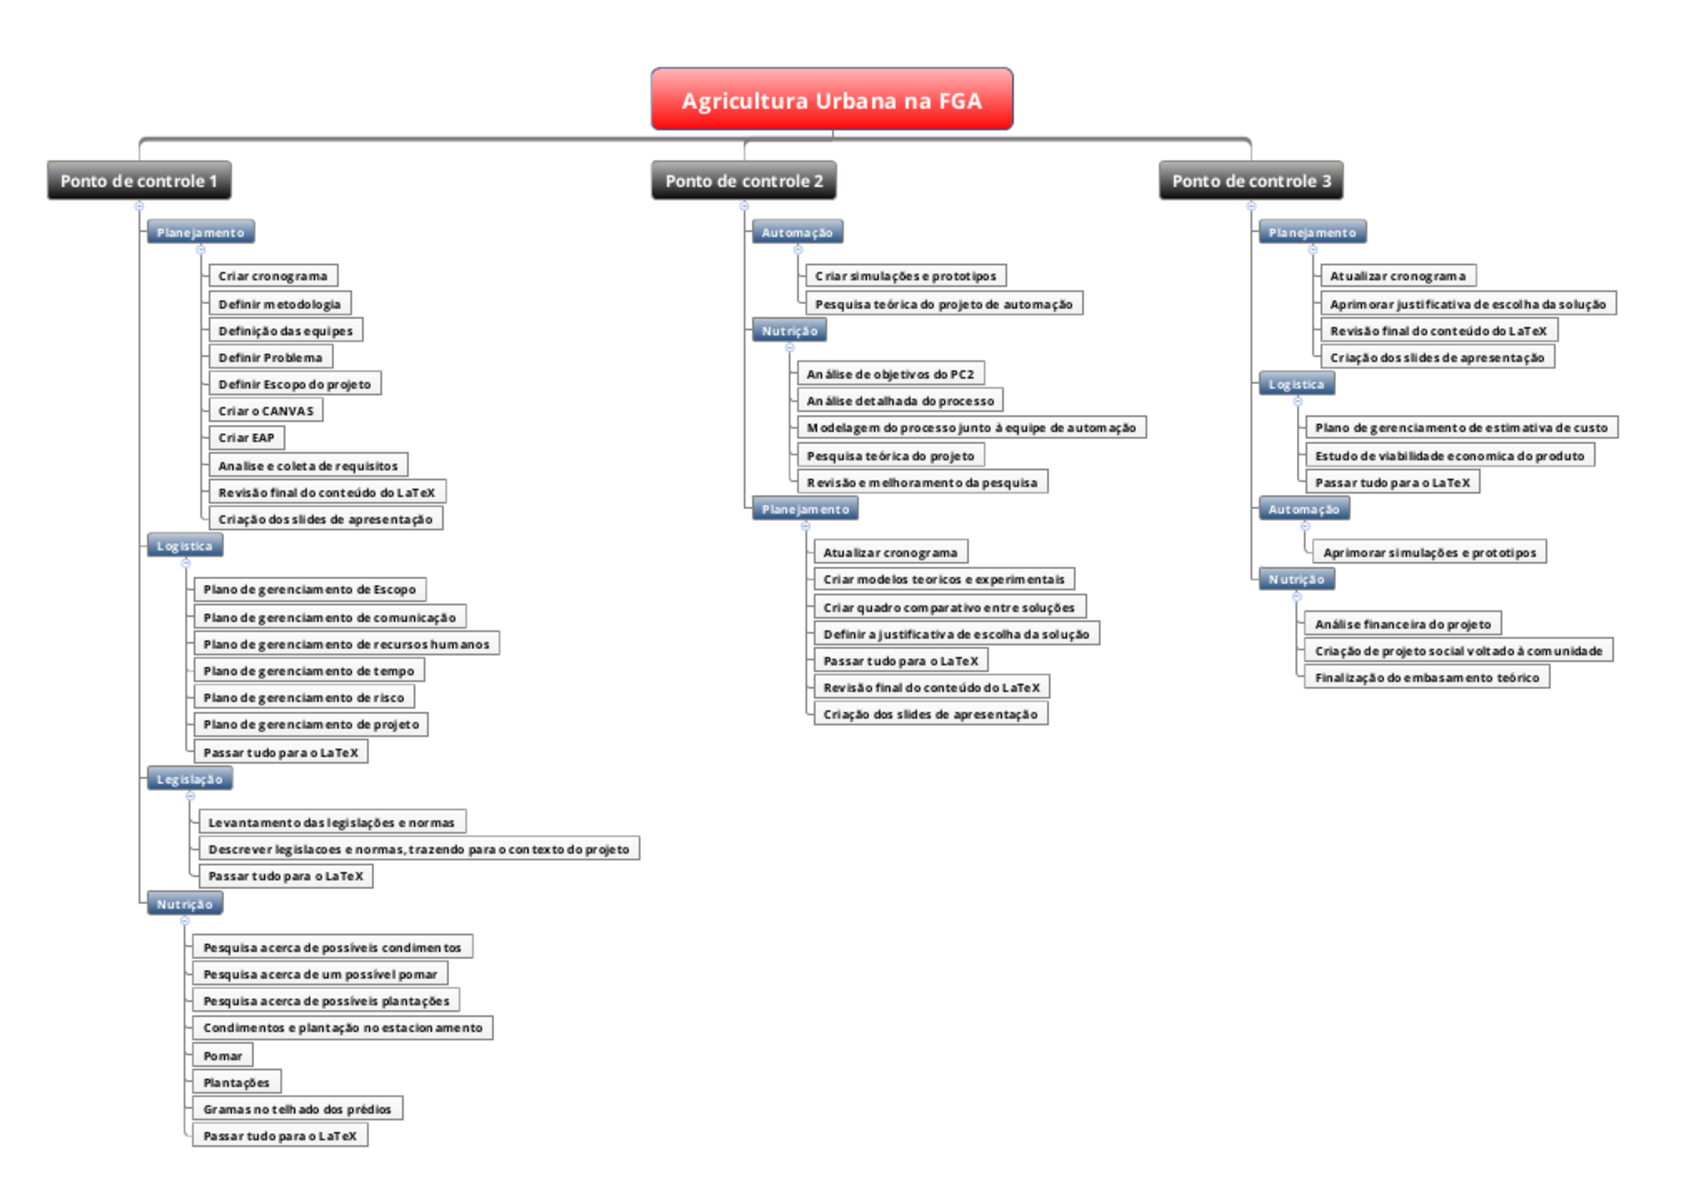
\includegraphics[width=17cm, keepaspectratio=true]{figuras/tempo/eap.eps}
    \caption{EAP do projeto}
  \end{figure}

  \begin{figure}[!htb]
    \centering
    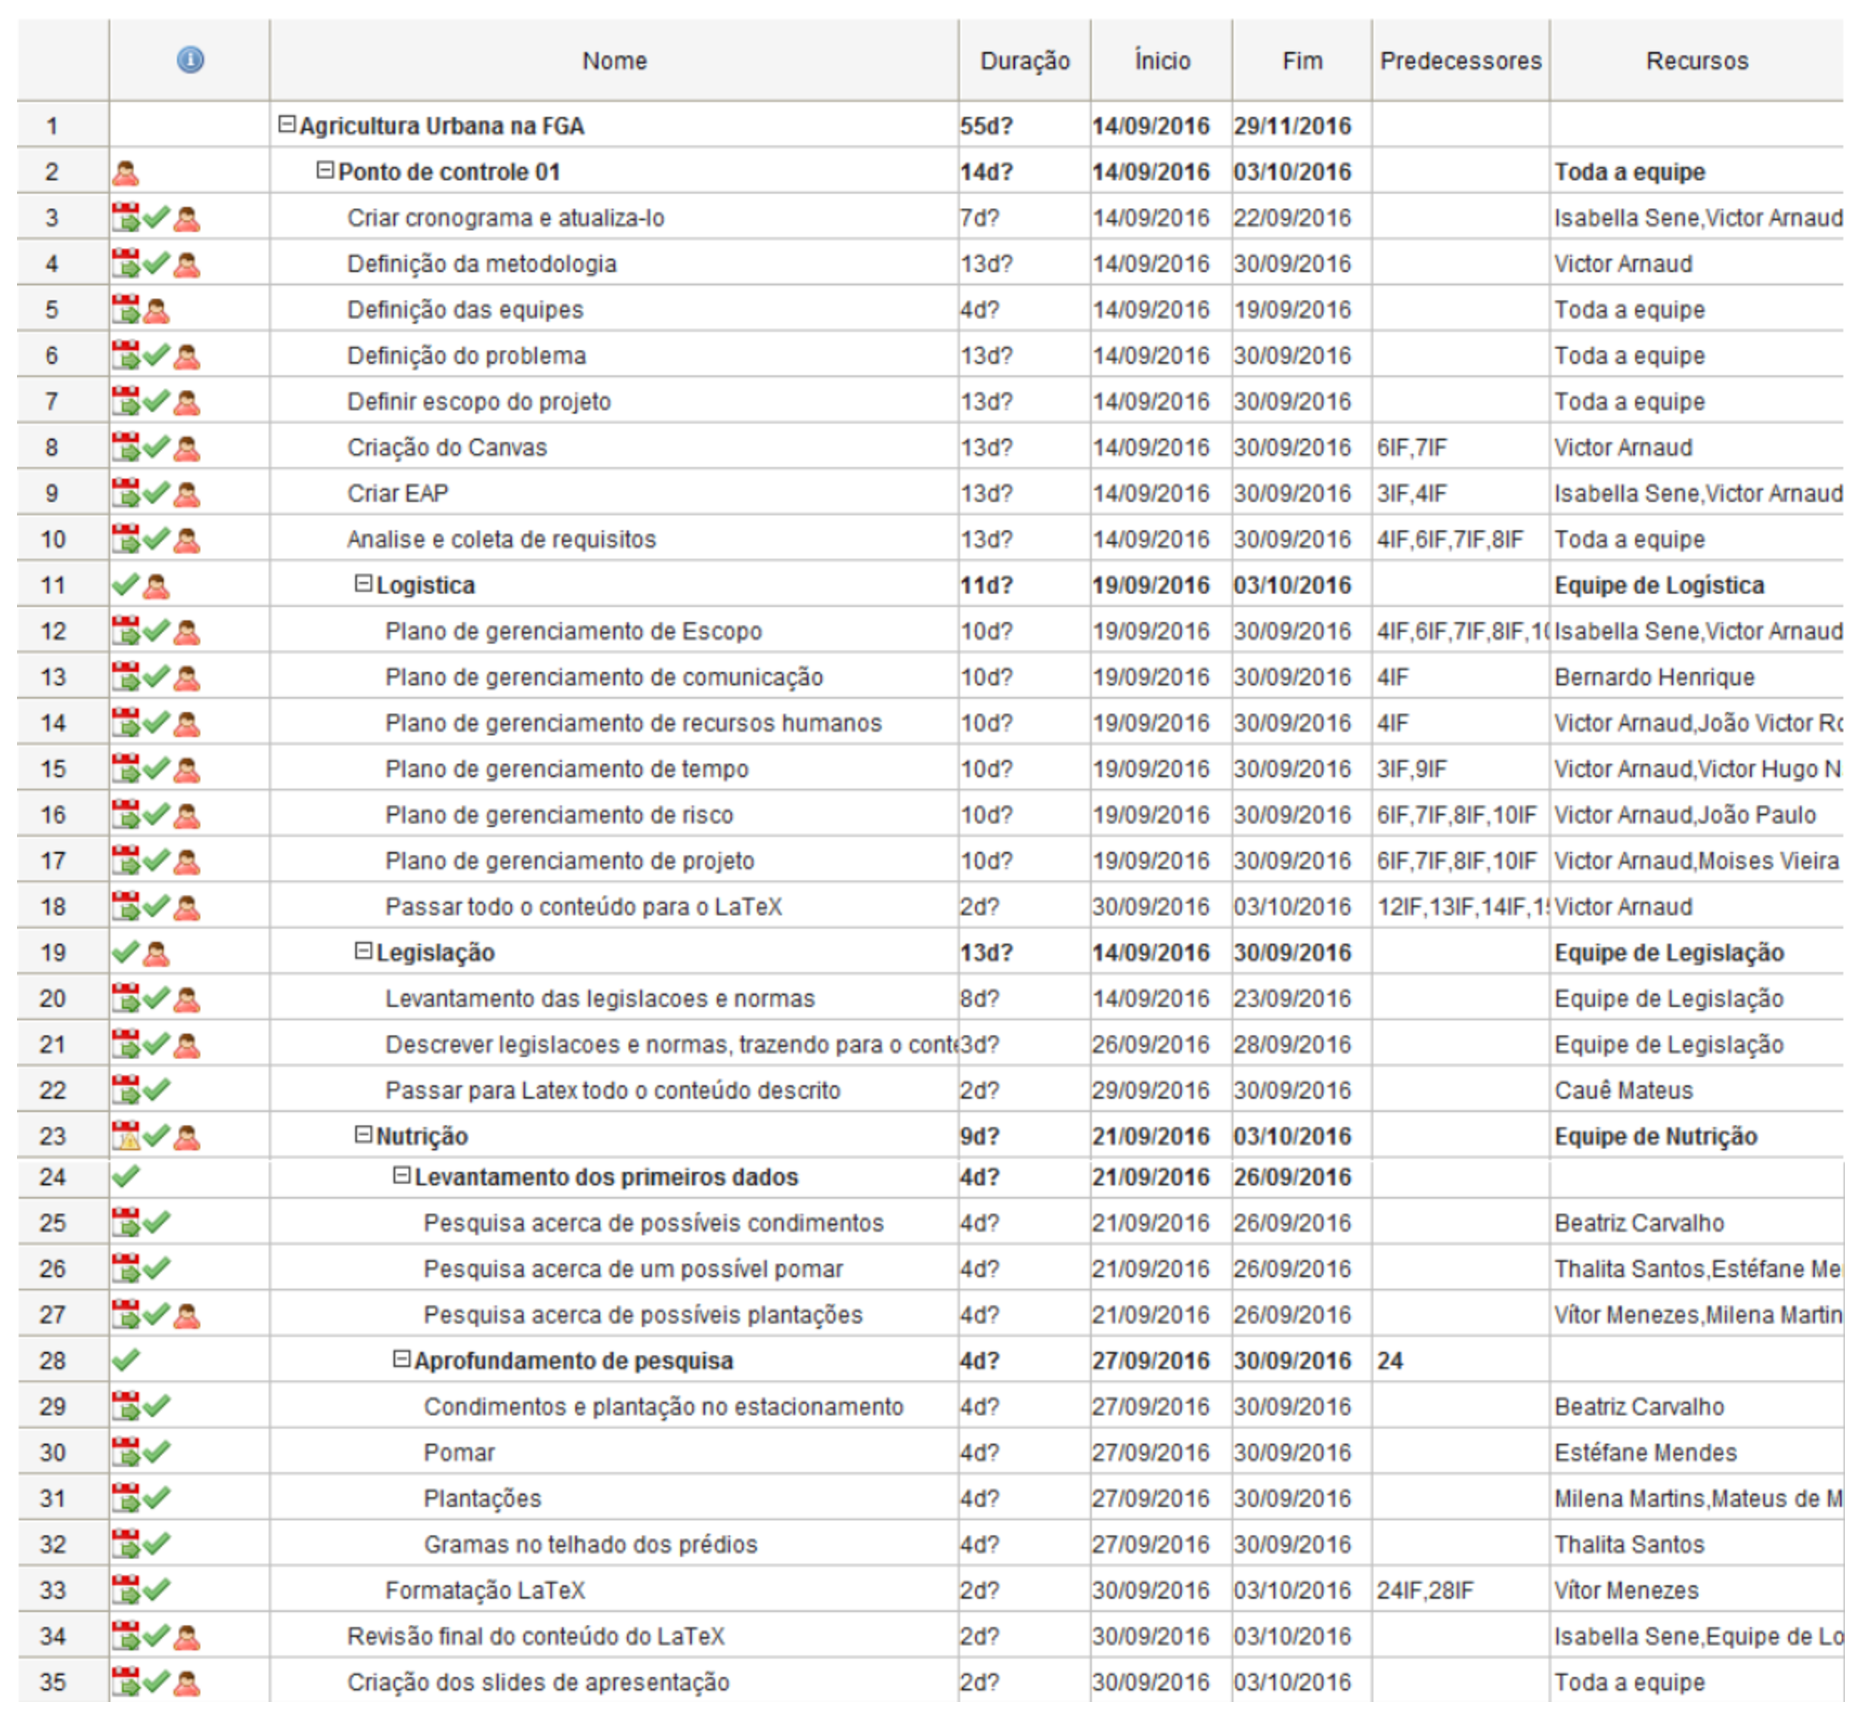
\includegraphics[width=15cm, keepaspectratio=true]{figuras/tempo/cronograma1.eps}
    \caption{Cronograma do ponto de controle 1}
  \end{figure}

  \begin{figure}[!htb]
    \centering
    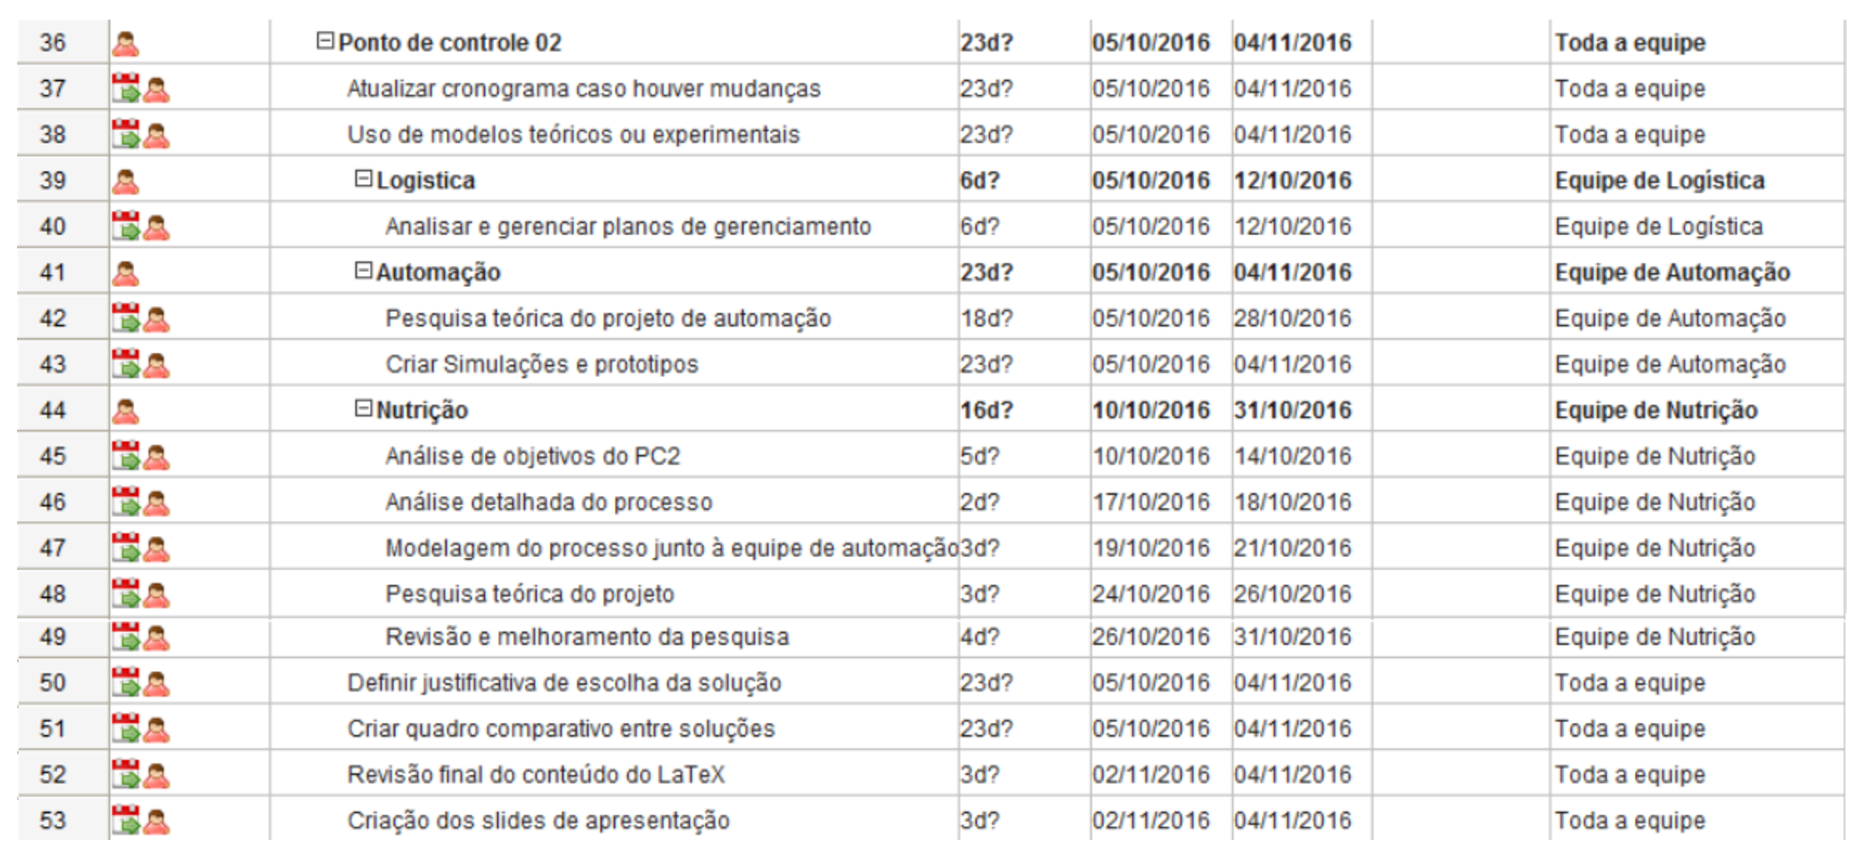
\includegraphics[width=15cm, keepaspectratio=true]{figuras/tempo/cronograma2.eps}
    \caption{Cronograma do ponto de controle 2}
  \end{figure}

  \begin{figure}[!htb]
    \centering
    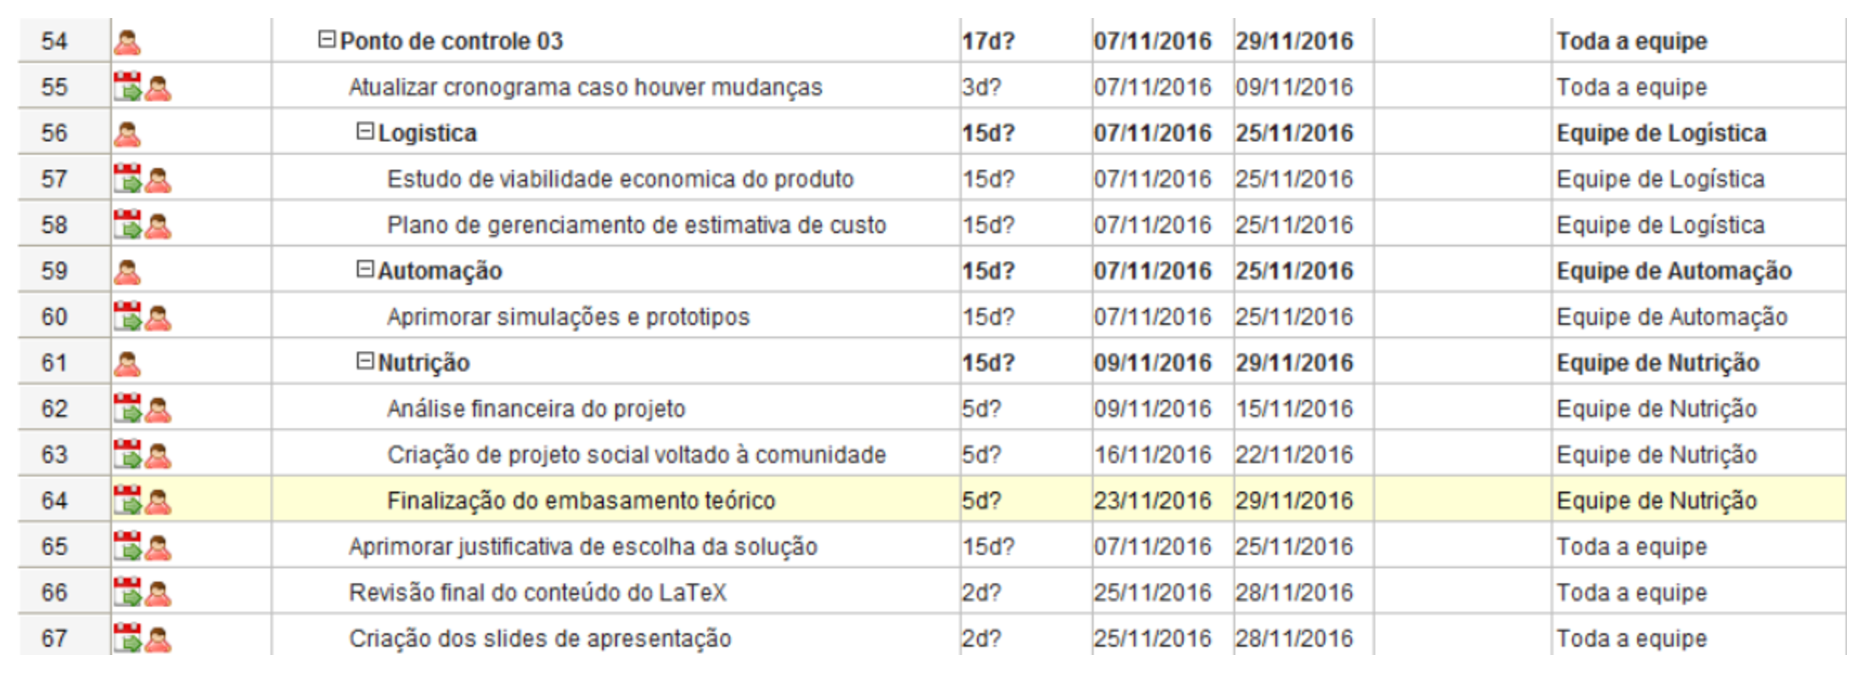
\includegraphics[width=15cm, keepaspectratio=true]{figuras/tempo/cronograma3.eps}
    \caption{Cronograma do ponto de controle 3}
  \end{figure}


\chapter{Plano de gerenciamento de risco}

  \label{risco}

  \section{Objetivo}

  Tem como objetivo a identificação dos possíveis riscos envolvidos no projeto, tal como os planos para tratamento.

\section{Riscos}

  Todos os riscos já identificados e futuros riscos serão documentados e apresentados neste documento, contendo suas
  características e possíveis soluções.

\subsection{Processo de gerenciamento de riscos}

  Visa definir um processo para qual os membros da equipe de gerência devem seguir para controle dos riscos no projeto.

  \begin{table}[!htb]
    \centering
    \begin{tabular}{p{5cm}p{10cm}}
      \toprule
        \textbf{Processo} & \textbf{Descrição} \\
      \midrule
        Identificar riscos  & Visa identificar os riscos que podem atrapalhar o projeto                                         \\ \midrule
        Analisar riscos     & Visa planejar como os riscos que possam vir ocorrer serão controlados ou resolvidos.              \\ \midrule
        Controlar riscos    & Visa acompanhar os riscos durante o período do projeto, avaliando a forma de resolução dos mesmos
                              durante toda a vida útil do projeto.                                                              \\
      \bottomrule
    \end{tabular}
    \caption{Processo de gerenciamento de risco}
  \end{table}

\subsection{Tabela dos riscos encontrados}

  Todos os riscos encontrados que podem prejudicar de alguma forma o projeto.

  \begin{table}[!htb]
    \centering
    \begin{tabular}{p{5cm}p{5cm}p{5cm}}
      \toprule
        \textbf{Risco} & \textbf{Impacto} & \textbf{Principal causa} \\
      \midrule
        Greve da UnB                                                    & Cronograma do projeto afetado                                   & Professores ou alunos insatisfeitos                                                   \\ \midrule
        Desistência ou falta de comprometimento de membros do projeto   & Atividades precisarão ser realocadas entre os membros restantes & Desmotivação dos alunos com a disciplina                                              \\ \midrule
        Falha no planejamento do projeto                                & Projeto entregue incompleto no ponto de controle seguinte       & Inexperiência da equipe de gerência                                                   \\ \midrule
        Mudanças no escopo                                              & Ajustes em toda a documentação do projeto                       & Falha de planejamento por partes dos alunos ou solicitação por parte dos professores  \\ \midrule
        Não cumprimento do escopo estabelecido                          & Projeto final faltando informações                              & Falta de maturidade da equipe do projeto                                              \\ \midrule
        Atraso na entrega dos documentos para a elaboração do relatório & Diminuição da nota do projeto                                   & Falta de comprometimento por parte dos membros                                        \\ \midrule
        Plágio nos relatórios                                           & Diminuição da credibilidade do relatório                        & Falta de comprometimento por parte dos membros                                        \\ \midrule
        Legislação não permitir realizar certas tarefas                 & Terá que fazer mudanças no escopo do projeto                    & Restrições estabelecidas pelas leis                                                   \\
      \bottomrule
    \end{tabular}
    \caption{Tabela de riscos do projeto}
  \end{table}

\newpage

\section{Qualificação dos riscos}

\subsection{Probabilidade de impacto dos riscos}

  A seguir está a probabilidade de impacto dos riscos

  \begin{table}[!htb]
    \centering
    \begin{tabular}{p{5cm}p{3cm}p{3cm}}
      \toprule
        \textbf{Probabilidade} & \textbf{Intervalo} & \textbf{Peso} \\
      \midrule
        Muito baixo & 0 $-$ 20\%    & 1 \\ \midrule
        Baixo       & 21 $-$ 40\%   & 2 \\ \midrule
        Moderado    & 41 $-$ 60\%   & 3 \\ \midrule
        Alta        & 61 $-$ 80\%   & 4 \\ \midrule
        Muito alta  & 81 $-$ 100\%  & 5 \\
      \bottomrule
    \end{tabular}
    \caption{Probabilidade de impacto dos riscos}
  \end{table}

  O impacto mede o quão prejudicial um risco é ao projeto como um todo, a seguir, está demonstrado como o impacto será representado.

  \begin{table}[!htb]
    \centering
    \begin{tabular}{p{3cm}p{5cm}p{2cm}}
      \toprule
        \textbf{Impacto} & \textbf{Descrição} & \textbf{Peso} \\
      \midrule
        Muito baixo & Impacto no projeto não é expressivo           & 1 \\ \midrule
        Baixo       & Impacto pouco expressivo                      & 2 \\ \midrule
        Moderado    & Pode prejudicar o projeto de maneira moderada & 3 \\ \midrule
        Alta        & Prejudica o andamento do projeto              & 4 \\ \midrule
        Muito alta  & Prejudica gravemente o andamento do projeto   & 5 \\
      \bottomrule
    \end{tabular}
    \caption{Qual prejudicial é o nível do impacto}
  \end{table}

\section{Matriz de probabilidade de impacto}

  É utilizada para mapear os riscos de acordo com sua probabilidade de ocorrer e impacto no projeto, dando maior visão do que deve ser
  priorizado pela equipe.

  \begin{table}[!htb]
    \centering
    \begin{tabular}{cp{2cm}p{2cm}p{2cm}p{2cm}p{2cm}}
      \toprule
        \textbf{Probabilidade/Impacto} & \textbf{1} & \textbf{2} & \textbf{3} & \textbf{4} & \textbf{5} \\
      \midrule
        \textbf{1} & 1 & 2  & 3  & 4  & 5  \\ \midrule
        \textbf{2} & 2 & 4  & 6  & 8  & 10 \\ \midrule
        \textbf{3} & 3 & 6  & 9  & 12 & 15 \\ \midrule
        \textbf{4} & 4 & 8  & 12 & 16 & 20 \\ \midrule
        \textbf{5} & 5 & 10 & 15 & 20 & 25 \\
      \bottomrule
    \end{tabular}
    \caption{Matriz de probabilidade de impacto}
  \end{table}

  Com o resultado da matriz de probabilidade, temos a seguinte estratégia de gerenciamento de riscos.

  \begin{itemize}
    \item \textbf{Aceitação do risco}: Não fazer nada a respeito do risco, porém tentar resolver o problema que será gerado no projeto,
      isso significa que se o problema realmente acontecer, você vai lidar com ele, em vez de antecipar  qualquer esforço para impedir
      que ocorra.
    \item \textbf{Mitigação do risco}: Limitar o impacto de um risco agindo antes dele acontecer.
    \item \textbf{Prevenção do risco}: Evitar completamente o risco, trata-se de fazer mudanças (às vezes drásticas) em seu plano do
      projeto e cronograma, para evitar o problema em potencial.
  \end{itemize}

  \begin{table}[!htb]
    \centering
    \begin{tabular}{p{5cm}p{5cm}p{5cm}}
      \toprule
        \textbf{Nível de prioridade} & \textbf{Intervalo da matriz} & \textbf{Ação a ser tomada} \\
      \midrule
      Baixo & 1 $-$ 5   & Aceitação do risco \\ \midrule
      Médio & 6 $-$ 14  & Mitigação do risco \\ \midrule
      Alto  & 15 $-$ 25 & Prevenção do risco \\
      \bottomrule
    \end{tabular}
    \caption{Ação a ser tomada no risco}
  \end{table}

\section{Controle de riscos}

  \begin{figure}[!htb]
    \centering
    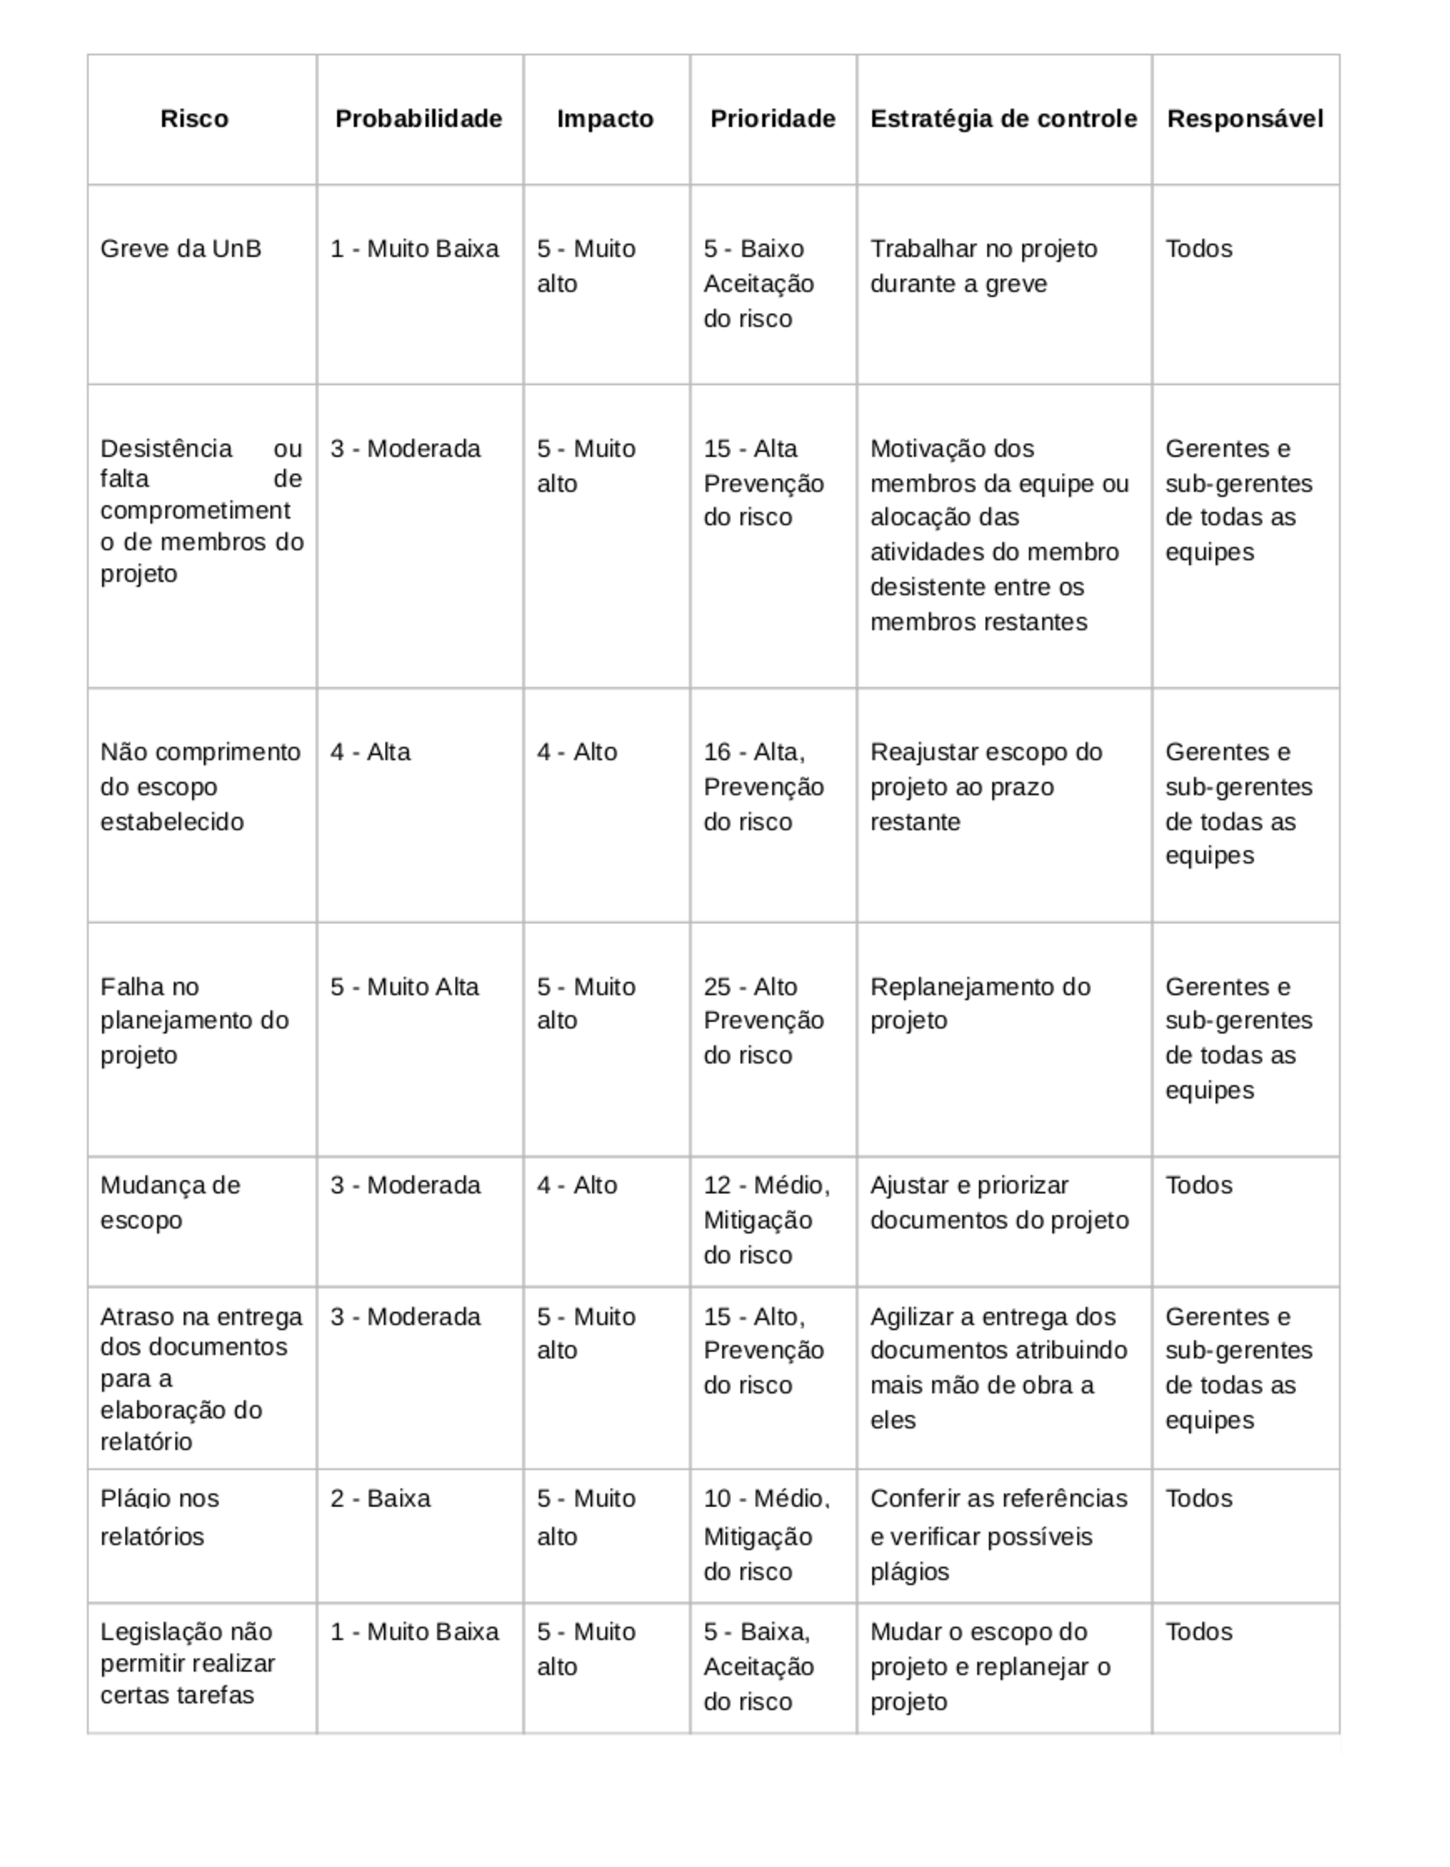
\includegraphics[width=15cm, keepaspectratio=true]{figuras/risco/risco.eps}
    \caption{Controle de riscos}
  \end{figure}



\chapter{Áreas Potenciais}

  \label{areas-potenciais}
  \begin{figure}[!htb]
    \centering
    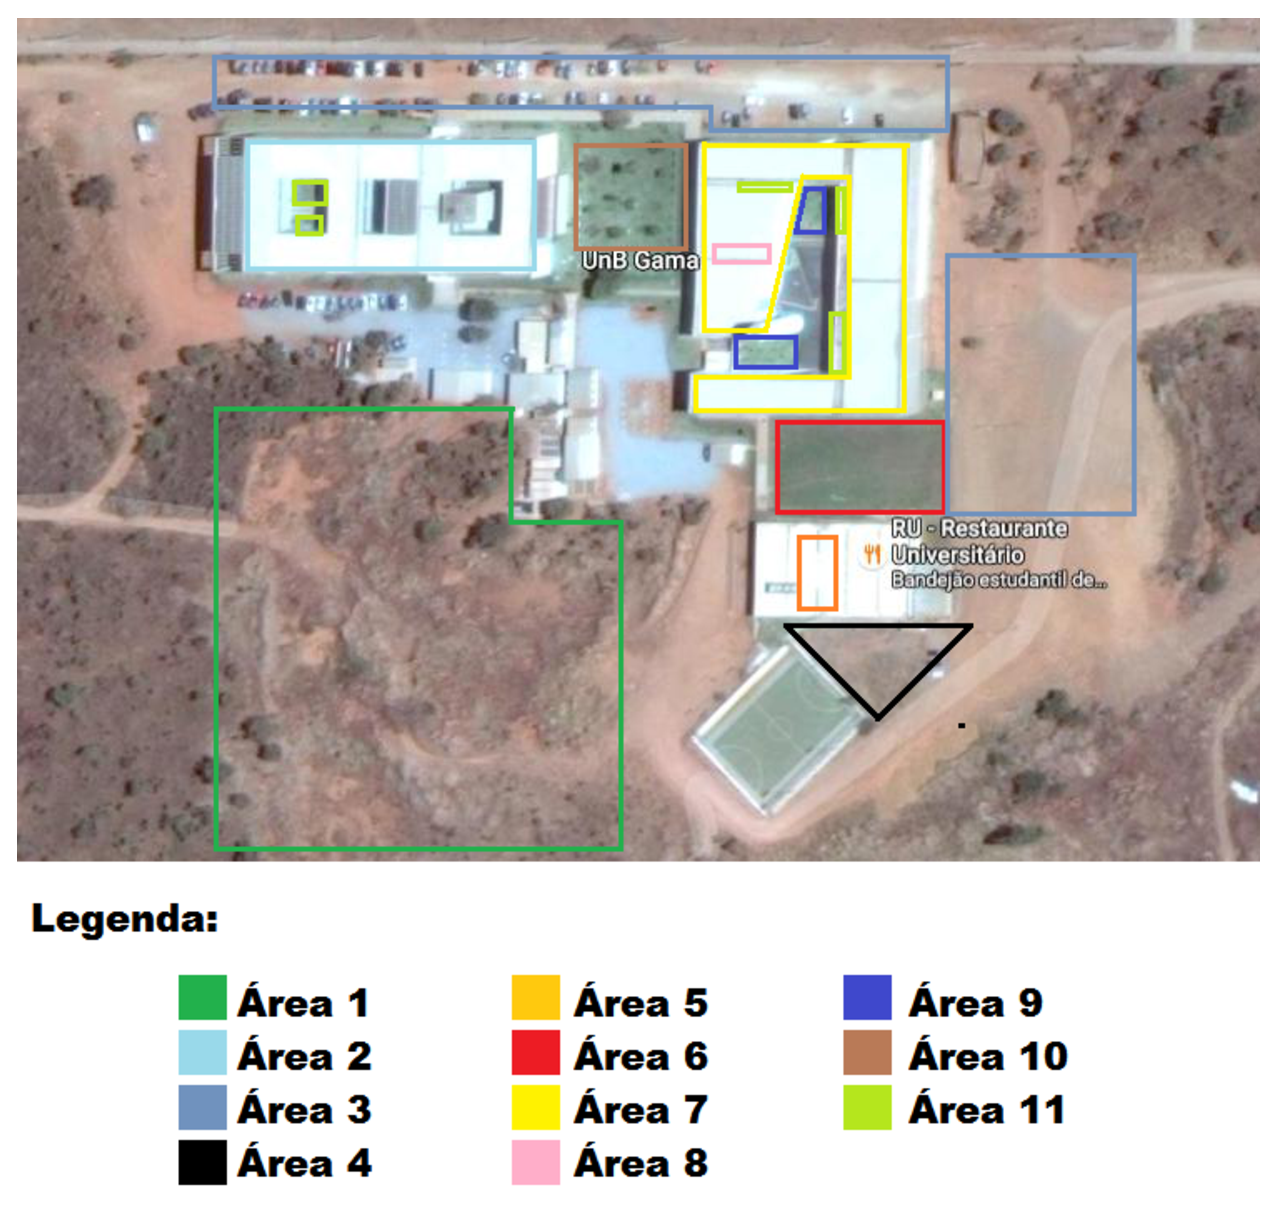
\includegraphics[width=12cm, keepaspectratio=true]{figuras/infraestrutura/fga.eps}
    \caption{Áreas potenciais para plantio}
  \end{figure}

  Figura criada a partir da imagem disponível no Google Maps \cite{infra1}.

\chapter{Tipos de solo no DF}

  \label{tipos-solo}
  \begin{figure}[!htb]
    \centering
    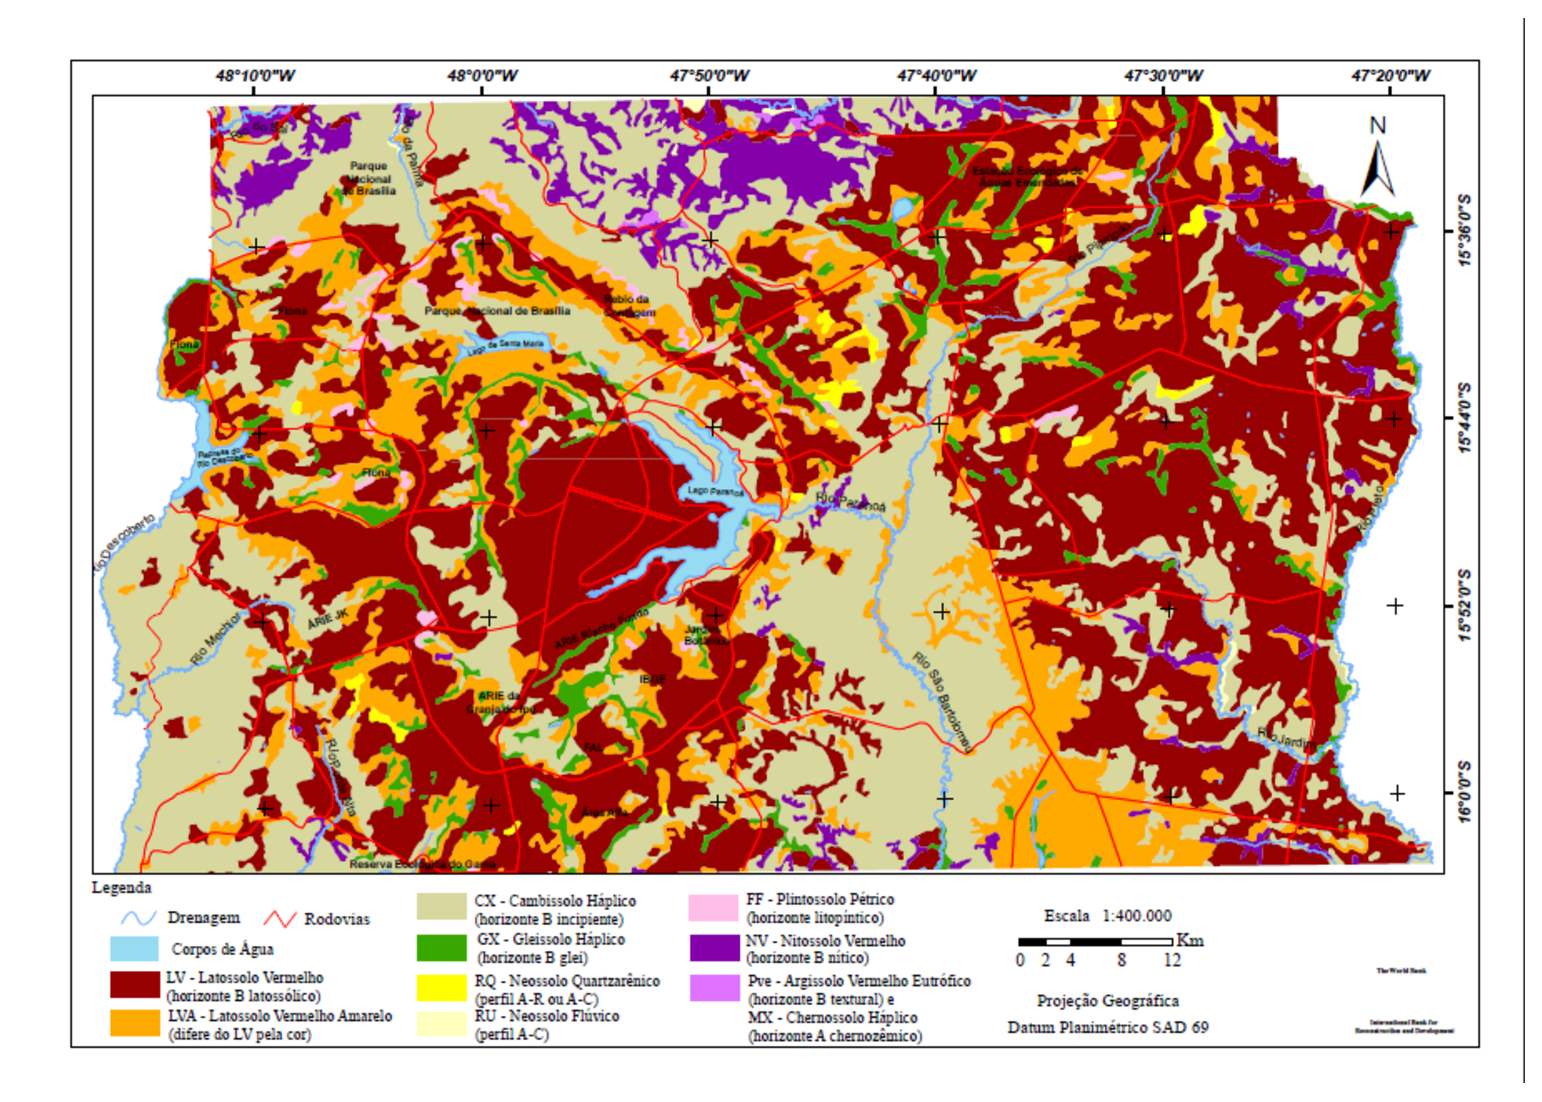
\includegraphics[width=12cm, keepaspectratio=true]{figuras/infraestrutura/solo.eps}
    \caption{Tipos de solo no Distrito Federal $-$ Fonte: Adasa}
  \end{figure}

\end{anexosenv}
